% Architecture slides (2 slides)
\section{Architecture}

% --- Slide 1: Architecture Notes ---
\begin{frame}{Architecture Overview}
\large
\begin{itemize}
  \item \textbf{Two-tier} network: edge nodes + central hub
  \item Edge nodes: piezo sensor + LM393 + ESP32 V1
  \item Hub: always-on ESP32, \textbf{[TODO]} bridges to cloud via Wi-Fi
  \item Communication: \textbf{ESP-NOW} (node $\rightarrow$ hub)
  \item Cloud: \textbf{[TODO]} \textbf{MQTT} broker + web dashboard
\end{itemize}

\vspace{0.4cm}
\begin{block}{Design Principle}
\large Sense and classify at the edge, act at the hub.
\end{block}
\end{frame}

% --- Slide 2: Detailed State Diagram ---
{
\setbeamertemplate{headline}{}
\setbeamertemplate{footline}{}
\begin{frame}[plain]{Sensor Node State Machine}
\begin{tikzpicture}[remember picture, overlay]
  \node[anchor=center] at (current page.center) {%
    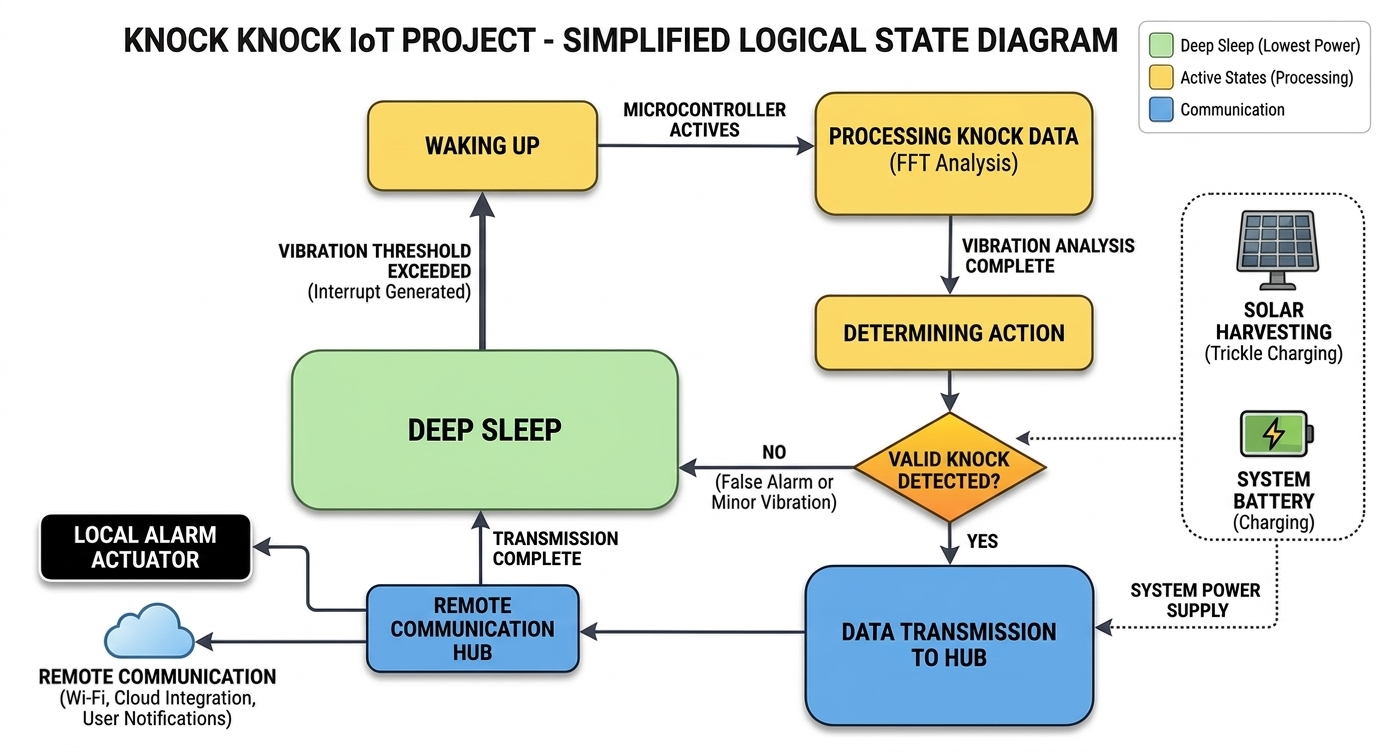
\includegraphics[width=0.96\paperwidth,height=0.92\paperheight,keepaspectratio]{images/project_schema.png}%
  };
\end{tikzpicture}
\end{frame}
}
